%%%%%%%%%%%%%%%%%%%%%%%%%%%%%%%%%%%%%%%%%%%%%%%%%%%%%%%%%%%%%%%%%%%%%%%%%%%%%%%%
\documentclass[12pt]{extarticle}
%%%%%%%%%%%%%%%%%%%%%%%%%%%%%%%%%%%%%%%%%%%%%%%%%%%%%%%%%%%%%%%%%%%%%%%%%%%%%%%%
\usepackage{fontspec}
\usepackage{polyglossia}
\usepackage[a4paper, lmargin=30mm, rmargin=15mm, tmargin=20mm, bmargin=20mm]{geometry}
\usepackage{multirow}

\setdefaultlanguage{russian}
\setotherlanguage{english}

\defaultfontfeatures{Ligatures=TeX}

\setmainfont{Times New Roman}
\setmonofont{Courier New}
\setsansfont{Arial}

\newfontfamily\cyrillicfont{Times New Roman}
\newfontfamily\cyrillicfontsf{Arial}
\newfontfamily\cyrillicfonttt{Courier New}

\newfontfamily\englishfont{Times New Roman}
\newfontfamily\englishfontsf{Arial}
\newfontfamily\englishfonttt{Courier New}

\linespread{1.5}

\usepackage[backend=biber,
  bibencoding=utf8,
  sorting=none,
  style=gost-numeric,
  language=autobib,
  autolang=other,
  clearlang=true,
  defernumbers=true,
  sortcites=true,
  doi=true,
  isbn=true,
  ]{biblatex}

\usepackage[dvipsnames]{xcolor}
\usepackage[
  hidelinks,
  colorlinks=true,
  linkcolor=Blue, % This is the color of table of contents and figure references
  citecolor=Blue, % This is the color of citations
  urlcolor=Blue % This is the colro of urls
]{hyperref}
\renewcommand{\UrlFont}{\small\rmfamily\tt}

\renewcommand\thesection{\arabic{section}}

\usepackage{amsfonts}
\usepackage{amsmath}

\usepackage{graphicx}
\graphicspath{ {./images/} } % This sets path to directory containing images.
\addto\captionsrussian{\renewcommand{\figurename}{Рисунок}} % This changes caption from 'Рис.' to 'Рисунок'.

%%%%%%%%%%%%%%%%%%%%%%%%%%%%%%%%%%%%%%%%%%%%%%%%%%%%%%%%%%%%%%%%%%%%%%%%%%%%%%%%
\addbibresource{biblio/bibliography.bib}
%%%%%%%%%%%%%%%%%%%%%%%%%%%%%%%%%%%%%%%%%%%%%%%%%%%%%%%%%%%%%%%%%%%%%%%%%%%%%%%%
\begin{document}
%%%%%%%%%%%%%%%%%%%%%%%%%%%%%%%%%%%%%%%%%%%%%%%%%%%%%%%%%%%%%%%%%%%%%%%%%%%%%%%%
\begin{titlepage}
  \begin{center}
    \linespread{1}
    \small
    Федеральное государственное автономное образовательное учреждение\break высшего образования\par
    <<Московский физико-технический институт \break (национальный исследовательский университет)>>\par
    Физтех-школа Прикладной Математики и Информатики\par
    Центр обучения проектированию и разработке игр\par
  \end{center}
%
  {
    \small
    {\bf Направление подготовки / специальность}: 09.03.01 Информатика и вычислительная техника\newline
    {\bf Направленность (профиль) подготовки}: Компьютерные науки и инженерия
  }
%
  {
    \topskip0pt
    \vspace*{\fill}
    \begin{center}
      {\bf\Large УЛУЧШЕНИЕ ГЕНЕРАЦИИ ДВИЖЕНИЯ РЭГДОЛА}\par(бакалаврская работа)
    \end{center}
    \vspace*{\fill}
  }
%
  \hfill
  \begin{minipage}[t]{8cm}
    {\bf Студент: \newline}
    Москалев Никита Евгеньевич\newline
    \vspace{-3mm}
    \rule{8cm}{0.15mm}
    \centerline{\scriptsize\it (подпись студента)}\newline
%
    {\bf Научный руководитель: \newline}
    Козак Роман Александрович\newline
    \vspace{-3mm}
    \rule{8cm}{0.15mm}
    \centerline{\scriptsize\it (подпись научного руководителя)}
  \end{minipage}

  \vspace*{\fill}
  \begin{center}
    Москва 2024
  \end{center}
\end{titlepage}
\newpage
\setcounter{page}{2}
\vspace*{\fill}
\begin{abstract}
% TODO: Fill abstract!
\end{abstract}
\vspace*{\fill}
\newpage
\tableofcontents
\newpage
\section{Введение}

Одна из основных задач, стоящих перед разработчиками и исследователями в области анимации, -- это воспроизведение разнообразия движений человека, с целью повышения реализма персонажей и их взаимодействий с игровым миром. Несмотря на сложности, связанные с недостаточным пониманием всех тонкостей движения человека, множество подходов к решению этой задачи было предложено за последние десятилетия, многие из которых в последствии были применены в разработке видео игр.

Существующие подходы можно разделить на две группы: основанные на данных \cite{AkikanFO}, \cite{KovarGP} и основанные на физическом моделировании \cite{AbeSP}, \cite{MacchiettoZS}, \cite{YinLP}. Такое разделение позволяет выделить ключевые идеи лежащие в основе многих из них, но не является исчерпывающим, поскольку существуют, например, гибридные подходы.

Подходы, составляющие первую группу, для создания анимаций персонажа используют большое количество предварительно записанных движений человека. Интенсивное развитие таких подходов началось после появления технологий оцифровки движений реальных объектов, таких как Motion Capture, позволивших существенно упростить сбор необходимых данных. Один из интересных примеров в этой группе -- это Motion Matching \cite{MotionMatching}. В нем анимация персонажа выбирается среди всех доступных каждый кадр. Критерии выбора могут быть разные -- вид движения, стилистика, направление. В сочетании с большой анимационной базой Motion Matching демонстрирует отличные результаты. Такие результаты обусловлены использованием данных, полученных из реального мира. Тем не менее это имеет и свои недостатки. В случае когда требуемое движение не стандартно или не может быть записано подходы основанные на данных плохо применимы.

Подходы, составляющие вторую группу, приводят персонажа в движение через управление динамикой его физической модели. В таком случае обеспечивается физическая корректность движения. Кроме того, при дополнительном моделировании окружающей персонажа среды появляется возможность обрабатывать взаимодействия с ней. К сожалению, из-за сложности разработки правил управления создание таких подходов является проблемой, также как и их использование, которое требует больших вычислительных ресурсов. Однако с углублением понимания механики движение человека и ростом производительности процессоров значимость этих недостатков будет уменьшаться. Поэтому генерация движения персонажа на основе физического моделирования остается перспективным направлением исследования.

Распространенная задача, возникающая при разработке систем управления персонажа, -- это необходимость поддержания баланса. Поддержание баланса подразумевает предотвращение неконтролируемого падения персонажа. Такая необходимость может возникнуть даже в самом простом случае, когда персонаж просто следует опорной анимации. А особенно ярко она проявляется, когда персонаж находится в присутствии внешних возмущений или на неровной поверхности. Кроме того, задача сильно варьирует в зависимости от вида воспроизводимого движения. Выделяют две категории баланса: статический, для движений на месте, и динамический.

В данной работе описывается и реализуется система управления персонажа, которая способна одновременно поддерживать баланс персонажа и следование персонажа опорной анимации. Поддержание баланса основано на контроле положений центра масс и центра давления. В каждый момент времени решается задача квадратичного программирования, которая оптимизирует значения целевых функций, отвечающих за контроль положений центра масс и центра давления и следование опорной анимации. После чего персонаж приводится в движение в  с результатами оптимизации. Более того, при изменение целевых функций описываемый способ может быть адаптирован для других задач, возникающих при разработке систем управления персонажем.

\subsection{Обзор литературы}

В данном разделе рассматриваются несколько работ, идеи из которых были заимствованы при разработке предлагаемой системы управления персонажем. Так же в таблице \ref{tbl:comparison_analysis} приведен их краткий сравнительный анализ.

\subsubsection{Dynamic Postural Adjustment with QP Method}

Похожая задача поддержания баласа возникает и в другой области -- робототехнике. Причем в отличие от анимаций, где целью является увеличение реалистичности и интерактивности персонажей, в робототехнике поддержание баланса робота критически важно для его успешного функционирования в реальных условиях. Из-за сходства методов физического моделирования персонажей и роботов, идеи, предложенные в области робототехники, могут быть применены в анимации, и наоборот.

Одно из первых применений контроля положений центра масс и центра давления было сделано в \cite{KudohKI}. В этой работе описывается алгоритм восстановления сбалансированного положения робота, после воздействия на него внешних возмущений. Основу алгоритма составляет вычисление обобщенных ускорений, таких чтобы центр масс возвращался в исходное положение, а центр давления, находился внутри допустимой области. Вычисление осуществляется применением одного из двух способов: оптимизации или пропорционально-дифференцирующего регулятора. Способ выбирается в зависимости от удаленности положения центра масс от исходного. Алгоритм демонстрирует движения робота схожие с теми, что выполняет человек для восстановления баланса. В дальнейшем алгоритм был доработан в \cite{MacchiettoZS} уже применительно к анимации.

\subsubsection{Multiobjective Control with Frictional Contacts}

В \cite{AbeSP} описывается система управления персонажем способная одновременно обеспечивать контроль положения центра масс и следование персонажа опорной анимации. В таком случае основную сложность составляет одновременная работа с несколькими целями движения, поскольку опорная анимация часто не является сбалансированной. Возможность учитывать несколько конфликтующих целей движения была получена применением оптимизации, целевая функция которой содержала вклад от каждой цели движения. Не смотря на то что работа фокусировалась только на контроле положения центра масс, что недостаточно для поддержания баласа во всех ситуациях, идея комбинирования целей движения открывает множество возможностей для дальнейшего улучшения.

\subsubsection{Momentum Control for Balance}

В \cite{MacchiettoZS} описывается система управления персонажем, которая контролирует положения центра масс и центра давления, а также обеспечивает следование персонажа опорной анимации. Работа с несколькими целями движения реализуется с помощью оптимизации, во время которой вычисляются оптимальные для текущей ситуации обобщенные ускорения. Полученные данные передаются в алгоритм обратной динамики, результаты которого вместе с внешними возмущениями используются алгоритмом прямой динамики для приведения персонажа в движение. Последние две стадии используются для того, чтобы интегрировать в систему внешние возмущения аналогично алгоритму, описанному в \cite{KudohKI}.

Отличительная особенностью системы, представленной в \cite{MacchiettoZS}, -- это использование импульса и момента импульса для контроля положений центра масс и центра давления. Такой способ также будет использован в данной работе.

\begin{table}[ht]
  \centering
  \begin{tabular}{ p{50mm} | p{26mm} | p{26mm} | p{26mm} }
    & Контроль положения ЦМ & Контроль положения ЦД & Следование опорной анимации \\
  \hline
  Dynamic Postural Adjustment with QP Method & Да & Нет & Нет \\
  \hline
  Multiobjective Control with Frictional Contacts & Да & Нет & Да \\
  \hline
  Momentum Control for Balance & Да & Да & Да \\
  \end{tabular}
  \caption{Сравнение рассмотренных работ}
  \label{tbl:comparison_analysis}
\end{table}

\subsection{Модель персонажа}

В данном разделе описывается физическая модель персонажа и формулируются уравнения, описывающие ее.

\subsubsection{Кинематическое дерево}

Кинематическое дерево -- это система из $n$ твердых тел, соединенных между собой $m$ шарнирами. Каждый из шарниров, кроме корневого, ограничивает относительное движение тел, которые он соединяет. Например, призматический шарнир оставляет только поступательное движение вдоль выбранной оси. Корневой шарнир, в свою очередь, определяет возможность системы перемещаться в пространстве и бывает двух видов: плавающий, то есть не накладывающий ограничений, и фиксирующий.

Для того чтобы приводить в движение отдельные тела, некоторые шарниры могут быть снабжены приводами, которые генерируют необходимые силы и моменты сил. В таком случае шарниры называется активными, иначе, соответственно, неактивными. Отметим, что корневой шарнир обычно остается неактивным. Таким образом за движение системы как целого отвечает сила трения. Это сохраняет физическую корректность, но сильно усложняет управление кинематическим деревом.

Работа системы управления такой моделью сводится к вычислению сил и моментов сил, которые должны генерировать приводы, чтобы получить движение удовлетворяющие заявленным требованиям, и последующему их применению, для воспроизведения движения.

В данной работе персонаж моделируется как кинематическое дерево, все шарниры которого имеют привод, причем силы и моменты сил, генерируемые в корневом шарнире, минимизируются во время оптимизации. Результаты показывают, что такая модель в большинстве ситуаций эквивалентна кинематическому дереву с неактивным корневым шарниром. На рисунках \ref{fig:visual_model} и \ref{fig:kinematic_tree} изображен пример трехмерной модели персонажа и соответствующего кинематического дерева.

\begin{figure}
  \begin{minipage}[t]{0.475\textwidth}
    \centering
    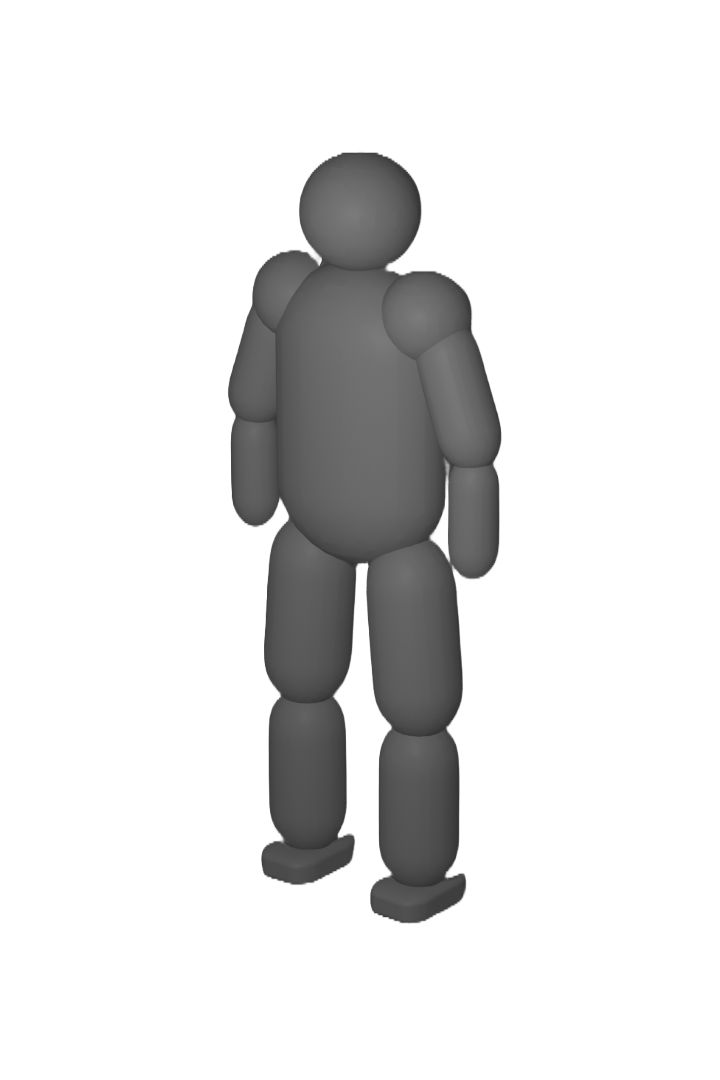
\includegraphics[scale=0.22]{visual_model.png}
    \caption{Трехмерная модель}
    \label{fig:visual_model}
  \end{minipage}
\hfill
  \begin{minipage}[t]{0.475\textwidth}
    \centering
    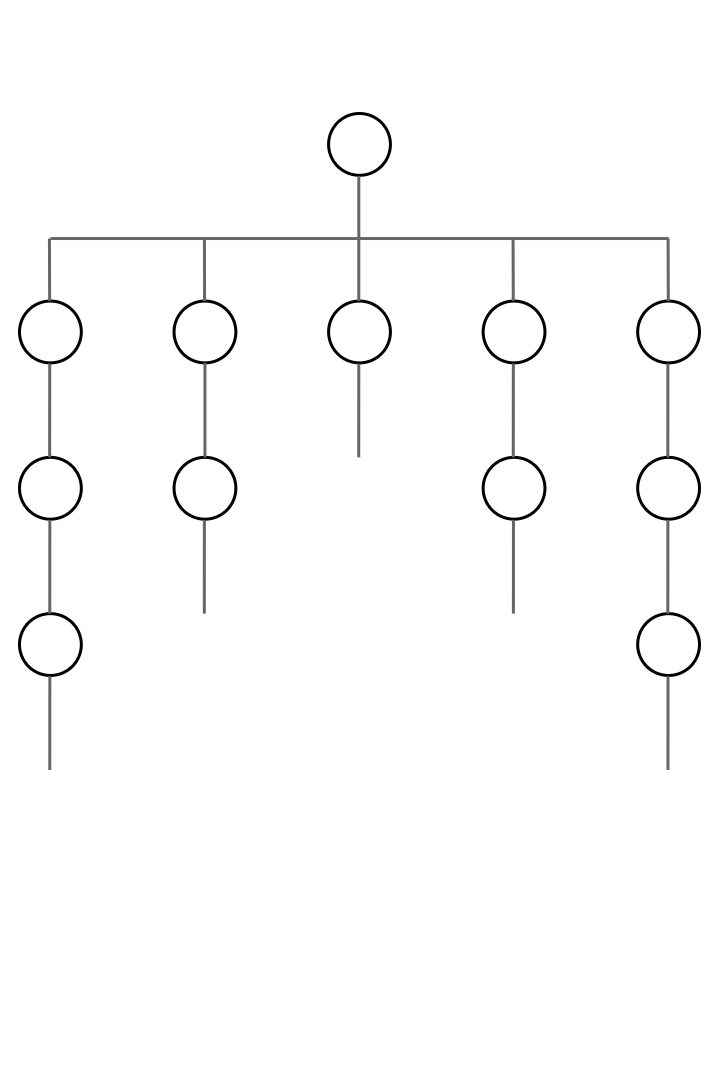
\includegraphics[scale=0.22]{kinematic_tree.png}
    \caption{Кинематическое дерево. Круги обозначают шарниры, а соединения между кругами -- твердые тела}
    \label{fig:kinematic_tree}
  \end{minipage}
\end{figure}

Отметим, что представление персонажа в виде кинематического дерева также называют активный рэгдол.

\subsubsection{Обобщенные координаты}

При работе с кинематическим дерево важную роль играет способ, выбранный для описания положения и ориентации тел в пространстве, поскольку он во многом определят простоту, устойчивость и вычислительную сложность моделирования. Основные способы -- это максимальные координаты и обобщенные координаты.

Максимальные координаты описывают тела по отдельности, используя по 6 чисел на каждое, а ограничения, накладываемые шарнирами, учитывают при решении уравнения динамики. Такой способ позволяет использовать существующие системы физического моделирования, но страдает от ошибок работы с вещественными числами, которые приводят к тому, что тела открепляются друг от друга.

Обобщенные координаты, напротив, учитывают связи между телами. Например, для кинематического дерева, состоящего из двух тел, соединенных вращательным шарниром, используется 7 чисел, первые 6 из которых описывают положение и ориентацию одного из тел, а оставшееся -- угол поворота вокруг оси шарнира. Такой способ минимизирует количество используемых чисел и неявно учитывает ограничения.

В данной работе используются обобщенные координаты, скорости и ускорения. Отметим, что обобщенные скорости позволяют выразить скорость любого шарнира. Для этого необходимо умножить их на якобиан шарнира. После чего можно получить скорость любой точки твердого тела, прикрепленного к шарниру, зная ее положение.

\subsubsection{Уравнение динамики}

Уравнение, связывающее обобщенные ускорения и силы и моменты сил, генерируемые приводами, называется уравнением динамики кинематического дерева и имеет вид
\begin{equation*}
  H \ddot{q} + C(q, \dot{q}) + G(q) = u + J^{T} f, \tag{1.1}\label{eq:1.1}
\end{equation*}
где $q, \dot{q}, \ddot{q}$ -- обобщенные координаты, скорости и ускорения, $H$ -- матрица инерции, $C$ -- центробежная и кориолисова силы, $G$ -- сила тяготения, $u$ -- силы и моменты сил, генерируемые приводами, $J$ -- якобиан, и $f$ -- внешние силы. Вывод этого уравнения из принципа наименьшего действия описан в \cite{Featherstone}.

В качестве неизвестной в уравнении \ref{eq:1.1} может выступать $\ddot{q}$ или $u$. Алгоритмы, которые находят $\ddot{q}$, называются алгоритмами прямой динамики, а те, которые находят $u$, -- обратной. Эффективные и повсеместно используемые реализации этих алгоритмов представлены в \cite{Featherstone}.

\subsubsection{Центроидальная матрица}

В \cite{OrinG} показана связь импульса и момента импульса кинематического дерева, выраженных в неподвижной системе отсчета, расположенной в центре масс, с обобщенными скоростями, имеющая следующий вид
\begin{equation*}
\begin{bmatrix} P\\ L \end{bmatrix} = A \dot{q}, \tag{1.2}\label{eq:1.2}
\end{equation*}
где $P$ -- импульс, $L$ -- момент импульса, а $A$ -- это центроидальная матрица.

Центроидальная матрица, как и матрицей инерции, является фундаментальной характеристикой кинематического дерева, которая зависит только от массы, инерции и значения обобщенных координат твердых тел, составляющих его.

При разделении центроидальной матрицы на две уравнение \ref{eq:1.2} принимает вид
\begin{align*}
  P &= A_{P} \dot{q}, \tag{1.3}\label{eq:1.3} \\
  L &= A_{L} \dot{q}. \tag{1.4}\label{eq:1.4}
\end{align*}

При дифференцировании уравнения \ref{eq:1.3} и \ref{eq:1.4} принимают вид
\begin{align*}
  \dot{P} &= \dot{A_{P}} \dot{q} + A_{P} \ddot{q}, \tag{1.5}\label{eq:1.5} \\
  \dot{L} &= \dot{A_{L}} \dot{q} + A_{P} \ddot{q}. \tag{1.6}\label{eq:1.6}
\end{align*}

Полученные уравнения \ref{eq:1.5} и \ref{eq:1.6} отражают связь между значениями производных импульса и момента импульса и обобщенными ускорениями. В данной работе они используются при формулировании целевой функции оптимизации.

\subsubsection{Импульс и момент импульса}

Положения импульса и момента импульса показывают устойчивость персонажа, поэтому одна из задач разрабатываемой системы управления -- это их контроль. Способ используемый в данной работе управляет импульсом и моментом импульса, таким образом контролируя положения центра масс и центра давления. В данном подразделе показана связь между этими величинами, которая обосновывает корректность выбранного способа.

Напомним, что центр давления -- это точка, где можно приложить результирующую сил нормальной реакции опоры и сил трения (далее -- силу реакции опоры), так чтобы момент относительно центра масс не изменился.

\begin{figure}[ht]
  \begin{minipage}{\textwidth}
    \centering
    \begin{tikzpicture}
      % character
      \node [rectangle, minimum width = 0.7cm, minimum height = 3.0cm, draw, fill = white, rotate around = {19:(1.4, -2.1)}] at (1.4, -2.1) {};
      \node [rectangle, minimum width = 0.7cm, minimum height = 2.6cm, draw, fill = white] at (-0.4, -2.7) {};
      \node [rectangle, minimum width = 0.7cm, minimum height = 2.4cm, draw, fill = white, fill opacity = 1.0] at (-0.4, -5.2) {};
      \node [rectangle, minimum width = 0.7cm, minimum height = 2.4cm, draw, fill = white, fill opacity = 1.0] at (1.26, -5.2) {};
      \node [rectangle, minimum width = 1.5cm, minimum height = 3.0cm, draw, fill = white, fill opacity = 1.0] at (0, 0) {};
      \node [circle, minimum width = 1.4cm, minimum height = 1.4cm, draw, fill = white, fill opacity = 1.0] at (0, 2.2) {};
      % ground
      \draw (-2, -6.4) -- (2.8, -6.4);

      % gravity
      \filldraw [fill = black] (0.1, -0.5) circle (2pt) node [above left] {$c$};
      \draw [-{Latex[length=4mm, width=2mm]}, line width = 0.5mm] (0.1, -0.5)  -- node[left] {$mg$} (0.1, -3.0);

      % ground reaction force
      \filldraw [fill = black] (0.2, -6.4) circle (2pt) node [below right] {$p$};
      \draw [-{Latex[length=4mm, width=2mm]}, line width = 0.5mm] (0.2, -6.4) -- node[right] {$f$} (0.8, -4.4);

    \end{tikzpicture}
    \caption{Силы}
    \label{fig:forces}
  \end{minipage}
\end{figure}

Рассмотрим силы, действующие на кинематическое дерево (рисунок \ref{fig:forces}). Запишем второй закон Ньютона и основное уравнение вращательной динамики
\begin{align*}
\dot{P} &= mg + f, \tag{1.7}\label{eq:1.7} \\
\dot{L} &= (p - c) \times f, \tag{1.8}\label{eq:1.8}
\end{align*}
где $c$ -- центр масс, $p$ -- центр давления, $m$ -- суммарная масса, и $f$ -- результирующая сил нормальной реакции опоры и сил трения.

Исключая $f$ из уравнений \ref{eq:1.7} и \ref{eq:1.8}, получим
\begin{equation*}
\dot{L} = (p - c) \times (\dot{P} - mg). \tag{1.9}\label{eq:1.9}
\end{equation*}

Полученное уравнение \ref{eq:1.9} показывает, что при известном импульсе и положении центра масс, контроль положения центра давления может быть сделан с помощью управления моментом импульса.

Теперь, запишем определение импульса кинематического дерева, рассматривая его как систему твердых тел
\begin{equation*}
  P = \sum_{i = 1}^{n} m_{i} \dot{x_{i}},
\end{equation*}
где $x_{i}$, $m_{i}$ -- положения и массы. Используя следующую цепочку равенств
\begin{equation*}
  \sum_{i = 1}^{n} m_{i} \dot{x_{i}} = \frac{d}{dt} (\sum m_{i} x_{i}) = \frac{d}{dt} (mc) = m \dot{c},
\end{equation*}
преобразуем уравнение к виду
\begin{equation}
  P = m \dot{c}, \tag{1.10}\label{eq:1.10}
\end{equation}
а дифференцированием к виду
\begin{equation}
  \dot{P} = m \ddot{c}. \tag{1.11}\label{eq:1.11}
\end{equation}

Полученное уравнения \ref{eq:1.11} показывает, что контроль ускорения центра масс может быть сделан с помощью управления производной импульса.
\section{Система управления персонажем}

Работа системы управления персонажем состоит из следующих стадий, повторяемых в цикле:
\begin{enumerate}
  \item оптимизация;
  \item прямая динамика;
  \item интегрирование.
\end{enumerate}

Во время оптимизации вычисляются силы и моментов сил, которые должны должны сгенерировать приводы, и силы реакции опоры, такие, чтобы получаемое движение было сбалансированным и следовало опорной анимации. Результаты оптимизации передаются в алгоритм прямой динамики, который находит ускорения. Далее скорости и ускорения интегрируются по временному шагу, с целью получения новых скоростей и обновления положения персонажа.

Внешние возмущения, если пресутсвуют, также передаются в алгоритм прямой динамики. Ошибки, которые они вносят в движение, компенсируются оптимизатором на следующих циклах работы системы.

На рисунке \ref{fig:architecture} схематично изображена работа системы.

\begin{figure}[ht]
  \begin{minipage}{\textwidth}
    \centering
    \begin{tikzpicture}
        \node [rectangle, minimum width = 4cm, minimum height = 3cm, draw] at (-6.0, 0.0) {Оптимизация};
        \node [rectangle, minimum width = 4cm, minimum height = 3cm, draw] at (0.0, 0.0) {Прямая динамика};
        \node [rectangle, minimum width = 4cm, minimum height = 3cm, draw] at (6.0, 0.0) {Интегрирование};
        \draw [-{Latex[length=3mm, width=2mm]}] (0.0, 3.5) -- node[right = 1mm] {$f_{d}$} (0.0, 1.5);
        \draw [-{Latex[length=3mm, width=2mm]}] (-4.0, 0.0)  -- node[above = 1mm] {$u, f$} (-2.0, 0.0);
        \draw [-{Latex[length=3mm, width=2mm]}] (2.0, 0.0)  -- node[above = 1mm] {$\ddot{q}$} (4.0, 0.0);
        \draw [-] (6.0, -1.5) -- (6.0, -3.5);
        \draw [-] (6.0, -3.5) -- node[below = 1mm] {$q, \dot{q}, \ddot{q}$} (-6.0, -3.5);
        \draw [-{Latex[length=3mm, width=2mm]}] (-6.0, -3.5) -- (-6.0, -1.5);
      \end{tikzpicture}
    \caption{Работа системы управления}
    \label{fig:architecture}
  \end{minipage}
\end{figure}

\subsection{Оптимизация}

Оптимизация -- это ключевая стадия работы системы управления, ответственная за вычисление сил и моментов сил, которые должны генерировать приводы, а также силы реакции опоры. Оптимизация выбрана поскольку она позволяет учесть все условия, влияющих на значения сил и моментов сил, в виде целевой функции или ограничений.

Задача оптимизации имеет следующий вид
\begin{align*}
  \min_{\ddot{q}, u, f} &\ \omega_{t} h_{t}(\ddot{q}) + \omega_{c} h_{c}(\ddot{q}) + \omega_{p} h_{p}(\ddot{q}) + \omega u^{T} \begin{bmatrix} I_{6} & O \\ O & O \end{bmatrix} u \\
  s.t. &\ H \ddot{q} + C(q, \dot{q}) + G(q) = u + J^{T} f \tag{2.1}\label{eq:2.1} \\
       &\ J_{sup} \ddot{q} + \dot{J}_{sup} \dot{q} = 0 \tag{2.2}\label{eq:2.2} \\
       &\ 0 \le n(f) \tag{2.3}\label{ineq:2.3} \\
       &\ \tau(f) \le \mu n(f) \tag{2.4}\label{ineq:2.4}
\end{align*}

Целевая функция оптимизации состоит из четырех слагаемых. Первые три из них -- $h_{t}$, $h_{c}$ и $h_{p}$ -- отвечают за следование опорной анимации, за положения центра масс и за положения центра давления соответственно. Последнее стремиться минимизировать силы и моменты сил, генерируемые в корневом шарнире. Веса $w_{t}$, $w_{c}$, $w_{p}$ и $w$ -- позволяют регулировать значимость вклада каждого из слагаемых.

Отметим, что последнее слагаемое важно для надежности и простоты настройки системы, поскольку оно обеспечивает обработку ситуаций, когда значения функций $h_{t}$, $h_{c}$ и $h_{p}$ значительно отклоняются от оптимальных и не могут быть восстановлены без генерации сил и моментов сил в корневом шарнире. Обычно вместо последнего слагаемого используется ограничение, требующее равенства сил и моментов сил в корневом шарнире нулю. Однако тогда система не может обработать ситуации выше. Применительно к анимациям в видео играх выбор в пользу надежности за счет возможной потери физической корректности может оказаться целесообразным.

Уравнение \ref{eq:2.1} согласует результаты оптимизации с уравнением динамики кинематического дерева. Таким образом, обобщенные ускорения, полученные применением алгоритма прямой динамики, в случае отсутствия внешних возмущений будут совпадать с теми, что найдены во время оптимизации. Уравнение \ref{eq:2.2} оставляет точки контакта с поверхностью неподвижными. Неравенства \ref{ineq:2.3} и \ref{ineq:2.4} отвечают за направление силы реакции опоры.

Функции $h_{t}$, $h_{c}$ и $h_{p}$ формулируются так, чтобы получившаяся задача оптимизации была квадратичной. Квадратичное программирование успешно применялось в других системах \cite{AbeSP}, \cite{MacchiettoZS}, \cite{SilvaAP}, поскольку оно дает дает предсказуемое время работы оптимизатора и воспроизводимые результаты.

Следующие подразделы посвящены функциям $h_{t}$, $h_{c}$ и $h_{p}$. Поскольку кинематическая характеристика, которую можно контролировать, -- это обобщенные ускорения, функции формулируются следующим образом: описывается желаемое ускорение, после чего определяется функция, оптимизация которой минимизирует отклонение получаемого ускорения от желаемого.

\subsubsection{Следование опорной анимацией}

Функция $h_{t}(\ddot{q})$ ответственна за поддержание стилистической составляющей движения, задаваемой с помощью опорной анимации. Основная задача этой функции в том, чтобы получаемое движение как можно точнее приближало опорную анимацию. Наивный способ добиться этого -- это взять $h_{t}(\ddot{q})$ такой, чтобы в результате оптимизации полученное ускорение совпадало ускорением из опорной анимации. Однако, в таком случае, если получаемое движение отклоняется от опорной анимации, например, в следствие внешних возмущений, то оно не будет скорректировано обратно. Поэтому функция $h_{t}(\ddot{q})$ включает слагаемые, которые характеризую отставание, и определяется следующим образом
\begin{equation*}
  h_{t}(\ddot{q}) = \lVert W (\ddot{q} + s_{t} (q - q_{ref}) + d_{t} (\dot{q} - \dot{q}_{ref}) - \ddot{q}_{ref}) \rVert_{2}^{2},
\end{equation*}
где $W$ -- диагональная матрица весов, $s_{t}$ и $d_{t}$ -- коэффициенты, а $q_{ref}$, $\dot{q}_{ref}$ и $\ddot{q}_{ref}$ -- это положение, скорость и ускорение взятые из опорной анимации. Матрица $W$ позволяет более точно настроить систему, сохранить требуемые особенностей опорной анимации. В данной работе матрица $W$ единичная.

Выражение $s_{t} (q - q_{ref}) + d_{t} (\dot{q} - \dot{q}_{ref})$ использованное в определении $h_{t}$ называется пропорционально-дифференцирующий регулятор (далее -- ПД регулятор), а коэффициенты $s_{t}$ и $d_{t}$ -- пропорциональный и дифференциальный соответственно. Одно из первых применений ПД регулятора для решения задачи следования физически моделируемого персонажа опорной анимации сделано в \cite{HodginsWBO}. Сейчас ПД регулятор -- это повсеместно используемая техника при разработке систем управления персонажем.

Отметим, что выбор коэффициентов $s_{t}$ и $d_{t}$ может существенно сказаться на результатах применения ПД регулятора. В данной работе коэффициенты удовлетворяют соотношению $d_{t} = \sqrt{s_{t}}$.

\subsubsection{Контроль положения центра масс}

Положение центра масс является хорошо известным индикатором баланса персонажа \cite{AbeSP}, \cite{MacchiettoZS}. В случае если проекция положения центра масс на поверхность находится вне опорного полигона (рисунок \ref{fig:support_polygon}), то есть выпуклой оболочки, образованной точками контакта с поверхностью, то персонаж может упасть. Таким образом, стратегия контроля положения центра масс состоит в том, чтобы поддерживать его проекцию на поверхность внутри опорного полигона, причем как можно дальше от границы.

\begin{figure}[ht]
  \begin{minipage}{\textwidth}
    \centering
    \begin{tikzpicture}
      \node [rectangle, minimum width = 1.5cm, minimum height = 2cm, draw, pattern=north east lines] at (1.5, 0.0) {};
      \node [rectangle, minimum width = 1.5cm, minimum height = 2cm, draw, pattern=north east lines] at (-1.5, 0.0) {};
      \node [rectangle, minimum width = 4.5cm, minimum height = 2cm, line width = 0.7mm, draw] at (0.0, 0.0) {};
      \filldraw [fill = black] (0.75, 1.0) circle (2pt) node [] {};
      \filldraw [fill = black] (2.25, 1.0) circle (2pt) node [] {};
      \filldraw [fill = black] (2.25, -1.0) circle (2pt) node [] {};
      \filldraw [fill = black] (0.75, -1.0) circle (2pt) node [] {};
      \filldraw [fill = black] (-0.75, -1.0) circle (2pt) node [] {};
      \filldraw [fill = black] (-2.25, -1.0) circle (2pt) node [] {};
      \filldraw [fill = black] (-2.25, 1.0) circle (2pt) node [] {};
      \filldraw [fill = black] (-0.75, 1.0) circle (2pt) node [] {};
    \end{tikzpicture}
    \caption{Опорный полигон. Заштрихованные прямоугольники обозначают стопы. Точки -- это точки контакта с поверхностью. Жирным выделен опорный полигон}
    \label{fig:support_polygon}
  \end{minipage}
\end{figure}

Реализовать это можно по разному. Простая и при этом эффективная реализация -- это выбор функции $h_c(\ddot{q})$ такой, чтобы в результате оптимизации проекция положение центра масс двигалось в направлении центра опорного полигона. Более точно, такой, чтобы ускорение центра масс стремилось к следующему значению
\begin{equation*}
  \ddot{c}_{des} = - s_{c} (c - c_{ref}) - d_{c} (\dot{c} - \dot{c}_{ref}), \tag{2.6}\label{eq:2.6}
\end{equation*}
где $s_{c}$ и $d_{c}$ -- коэффициенты, а $c_{ref}$ и $\dot{c}_{ref}$ -- опорные положение и скорость центра масс. Такая формулировка желаемого ускорения центра масс делает контроль его положения более настраиваемым. В данной работе $c_{ref}$ выбрано как положение центра опорного полигона, а $\dot{c}_{ref}$ равно нулю. С другой стороны, $c_{ref}$ и $\dot{c}_{ref}$ могут быть взяты из опорной анимации. Отметим, что коэффициенты $s_{c}$ и $d_{c}$ могут быть константами или значениями, меняющимися в зависимости от состояния персонажа, как это сделано в \cite{AbeSP}.

Поскольку контроль положения центра масс вдоль гравитационной оси не важен для поддержания проекции центра масс на поверхность внутри опорного полигона, уравнение \ref{eq:2.6} рассматривается только по двум ортогональным гравитационной осям.

Преобразуем уравнение \ref{eq:2.6} к виду необходимому, чтобы сформулировать $h_c(\dot{q})$. Умножением обоих частей на массу, уравнение \ref{eq:2.6} принимает вид
\begin{equation*}
  m \ddot{c}_{des} = - s_{c} m (c - c_{ref}) - d_{c} m \dot{c}. \tag{2.7}\label{eq:2.7}
\end{equation*}
Подставляя $m \ddot{c}_{des}$ и $m \dot{c}$ из уравнений \ref{eq:1.10} и \ref{eq:1.11}, уравнение \ref{eq:2.7} принимает вид
\begin{equation*}
  \dot{P}_{des} = - s_{c} m (c - c_{ref}) - d_{c} P. \tag{2.8}\label{eq:2.8}
\end{equation*}
Подставляя $P$ из уравнения \ref{eq:1.3}, уравнение \ref{eq:2.8} принимает вид
\begin{equation*}
  \dot{P}_{des} = - s_{c} m (c - c_{ref}) - d_{c} A_{P} \dot{q}. \tag{2.9}\label{eq:2.9}
\end{equation*}

Функцию $h_c(\ddot{q})$ можно сформулировать как квадратичное отклонения получаемого импульса от желаемого импульса. Поскольку оптимизация происходит по переменным $\ddot{q}$, $u$, $f$ получаемый импульс необходимо выразить через обобщенные ускорения, используя уравнение \ref{eq:1.5}. Таким образом $h_c(\ddot{q})$ имеет вид
\begin{equation*}
  h_{c}(\ddot{q}) = \lVert A_{P}\ddot{q} - \dot{A_{P}} \dot{q} - P_{des} \rVert_{2}^{2}. \tag{2.10}\label{eq:2.10}
\end{equation*}

\subsubsection{Контроль положения центра давления}

Положение центра давления является индикатором вращательной устойчивости движения персонажа \cite{MacchiettoZS}, \cite{GoswamiK}. В случае если положение центра давления находится вне опорного полигона, то персонаж может опрокинуться. Кроме того, в случае если центр давления находится на границе опорного полигона, может возникнуть вращение опоры, то есть стоп персонажа. Таким образом, стратегия контроля положения центра давления состоит в том чтобы поддерживать его строго внутри опорного полигона.

Реализовать эту можно аналогично тому как сделан контроль положения цента масс. А именно, выбрать функцию $h_{p}(\ddot{q})$ такой, чтобы ускорения центра давления стремилось к следующему значению
\begin{equation*}
  \ddot{p}_{des} = - s_{p} (p - p_{ref}) - d_{p} (\dot{p} - \dot{p}_{ref}), \tag{2.11}\label{eq:2.11}
\end{equation*}
где $s_{p}$ и $d_{p}$ -- коэффициенты, а $p_{ref}$ и $\dot{p}_{ref}$ -- опорные положение и скорость центра давления. В данной работе $d_{ref}$ выбрано как положение центра опорного полигона, а $\dot{d}_{ref}$ равно нулю.

Преобразуем уравнение \ref{eq:2.11} к виду необходимому, чтобы сформулировать $h_p(\dot{q})$. Интегрируя $\ddot{p}_{des}$ получим значение $p_{des}$. Используя уравнение \ref{eq:1.9} получим
\begin{equation*}
  \dot{L}_{des} = (p_{des} - c) \times (P_{des} - mg). \tag{2.12}\label{eq:2.12}
\end{equation*}
Отметим, что при использовании уравнения \ref{eq:1.9} значение импульса взято из уравнения \ref{eq:2.9}, для того чтобы контроль положения центра давления был согласован с контролем положения центра масс.

Функцию $h_{p}(\ddot{q})$ можно сформулировать как квадратичное отклонения получаемого импульса от желаемого импульса. Поскольку оптимизация происходит по переменным $\ddot{q}$, $u$, $f$ получаемый импульс необходимо выразить через обобщенные ускорения, используя уравнение \ref{eq:1.5}. Таким образом $h_c(\ddot{q})$ имеет вид
\begin{equation*}
  h_{p}(\ddot{q}) = \lVert A_{L}\ddot{q} - \dot{A_{L}} \dot{q} - L_{des} \rVert_{2}^{2}. \tag{2.13}\label{eq:2.13}
\end{equation*}

\subsubsection{Положением точек контакта с поверхностью}

Положение точек контакта персонажа с поверхностью должны оставаться неподвижным, чтобы выполнялось условие нескользящего контакта.

Пусть имеется $k$ точек контакта с поверхностью пронумерованных от $1$ до $k$. Соответствующие якобианы, то есть матрицы, отображающие обобщенные скорости на скорости в пространстве, равны $J_{1}, \ldots, J_{k}$. Поэтому скорости точек контакта с поверхностью, обозначаемые $v_{1}, \ldots, v_{k}$, имеют следующий вид
\begin{equation*}
  \begin{bmatrix} v_{1} \\ \vdots \\ v_{k} \end{bmatrix} = \begin{bmatrix} J_{1} \\ \vdots \\ J_{k} \end{bmatrix} \dot{q}. \tag{2.14}\label{eq:2.14}
\end{equation*}
Обозначим столбец скоростей через $v_{sup}$, а столбец Якобианов -- $J_{sup}$. Тогда уравнение \ref{eq:2.14} приобретает вид
\begin{equation*}
  v_{sup} = J_{sup} \dot{q}. \tag{2.15}\label{eq:2.15}
\end{equation*}
Дифференцируя уравнение \ref{eq:2.15}, получаем выражение для ускорений $a_{sup}$ следующего вида
\begin{equation*}
  a_{sup} = J_{sup} \ddot{q} + \dot{J}_{sup} \dot{q}. \tag{2.16}\label{eq:2.16}
\end{equation*}

Для того чтобы скорости точек контакта с поверхностью оставались неподвижными, необходимо поддерживать ускорение равным нулю. Таким образом условие неподвижности точек контакта с опорой имеет следующий вид
\begin{equation*}
  J_{sup} \ddot{q} + \dot{J}_{sup} \dot{q} = 0. \tag{2.17}\label{eq:2.17}
\end{equation*}

\subsubsection{Направление силы реации опры}

Пусть функция $n(f): \mathbb{R}^{3} \rightarrow \mathbb{R}$ возвращает величину проекции $f$ на нормаль к поверхности, функция $\tau(f): \mathbb{R}^{3} \rightarrow \mathbb{R}$ возвращает величину проекции $f$ на поверхность.

Сила нормальной реакции -- это результирующая силы нормальной опоры и силы трения, каждая из которых имеет свои ограничениями. Сила нормальной реакции опоры всегда направлена вдоль нормали и не может быть отрицательной. Сила трения не превосходит силу нормальной реакции опоры умноженную на коэффициент трения, $\mu$. В терминах функции $n(f)$ и $\tau(f)$ эти ограничения формулируются в виде следующих неравенств
\begin{align*}
&\ 0 \le n(f), \tag{2.18}\label{ineq:2.18} \\
&\ \tau(f) \le \mu n(f). \tag{2.19}\label{ineq:2.19}
\end{align*}

\subsection{Прямая динамика}

Прямая динамика -- это стадия, во время которой происходит вычисление ускорений, которые далее вместе со скоростями будут проинтегрированы с целью обновления состояния персонажа. Наличие данной стадии в системе необходимо для возможности восстанавливать баланс в присутствии внешних возмущений. Поскольку величина внешних возмущений еще не известна на стадии оптимизации, она не может быть учтена на этой стадии. Поэтому оптимизация полагается на результаты прямой динамики, и корректирует их в соответствии с требованиями к движению.

Отметим, что если необходимости восстанавливать баланс в присутствии внешних возмущений нет, то можно сразу использовать ускорения, полученные во время оптимизации, поскольку они согласованы с уравнением динамики.

В данной работе используется алгоритм прямой динамики articulated rigid body, описанный в \cite{Featherstone}. Он выбран поскольку обладает наименьшей вычислительной сложность среди алгоритмов прямой динамики.

% \section{Результаты}

\section{Заключение}

В рамках проведенной работы была реализована система система управления персонажа, которая способна одновременно поддерживать баланс персонажа, основываясь на индикаторах баласа, таких как положение центр масс и положение центра давления, и следование персонажа опорной анимации. Были показаны успешные результаты применения данной системы. Кроме того, разработанная система обладает рядом полезных преимуществ. Во первых, система обладает высокой вариативностью с точки зрения визуальных результатов, поскольку имеет большое количество параметров, обеспечивающих возможность точной настройки. Во вторых, система обладает более простой настройкой, которую обеспечивает формулировка задачи оптимизации. В третьих, при система может быть адаптирована для для решения других задач, возникающих в области анимаций персонажа, основанных на физическом моделировании.

В дальнейшем планируется интегрировать реализованную систему в виде плагина в существующие игровые движки. Также планируется исследовать применимость системы в качестве анимационного фильтра, который преобразует несбалансированные анимации в сбалансированные. Кроме того, планируется реализовать данную систему на языке программирования C++ с целью повышения производительности.

\newpage
\printbibliography
%%%%%%%%%%%%%%%%%%%%%%%%%%%%%%%%%%%%%%%%%%%%%%%%%%%%%%%%%%%%%%%%%%%%%%%%%%%%%%%%
\end{document}
%%%%%%%%%%%%%%%%%%%%%%%%%%%%%%%%%%%%%%%%%%%%%%%%%%%%%%%%%%%%%%%%%%%%%%%%%%%%%%%%